\chapter{\ifproject%
\ifenglish Experimentation and Results\else การทดลองและผลลัพธ์\fi
\else%
\ifenglish System Evaluation\else การประเมินระบบ\fi
\fi}
\section{วัตถุประสงค์ของการทดสอบ}
\begin{enumerate}
    \item ทดสอบว่าผู้เล่นได้รับความสนุกสนานจากการเล่นเกม Witch Hunter
    \item ทดสอบการทำงานของระบบเกมว่าถูกต้องสมบูรณ์
\end{enumerate}
\section{การทดสอบความพึงพอใจในการเล่น}

ผู้พัฒนาได้ทดสอบเกมกับผู้เล่นจำนวน 10 คนในช่วงอายุ 20-23 ปี ซึ่งส่วนใหญ่เป็นผู้ที่คุ้นเคยกับการเล่นเกม Multiplayer Action-Horror
โดยให้ผู้เล่นจับกลุ่มกันและสลับบทบาทกันเล่น รวมถึงมีการสลับกลุ่มคละ ๆ กันระหว่างผู้ที่ชำนาญและไม่ชำนาญในการเล่นเกมนี้
ทั้งหมดนี้ก็เพื่อให้ได้ประสบการณ์เล่นที่ครบถ้วนและทดสอบความสมดุลของแต่ละฝั่งในเกม คะแนนความพึงพอใจในเล่นเกมมี 5 ระดับ:
1.ไม่พอใจที่สุด 2.ไม่พอใจ 3.พอใจ 4.พอใจมาก 5.พอใจมากที่สุด  ซึ่งผลลัพธ์ของการทดสอบความพึงพอใจเป็นดังนี้

\begin{figure}[h]
\begin{subfigure}{\textwidth}
    \begin{center}
    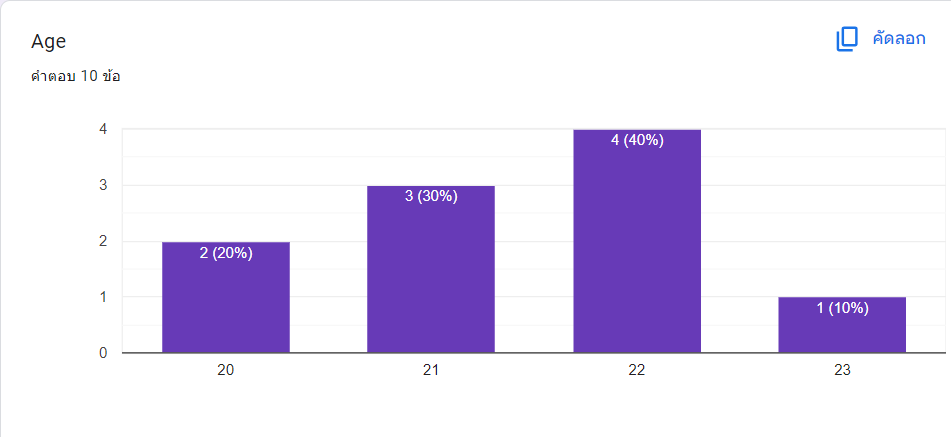
\includegraphics[width=0.8\textwidth]{./img/result/1.png}
    \label{fig:age}
    \end{center}
\end{subfigure}
\begin{subfigure}{\textwidth}
    \begin{center}
    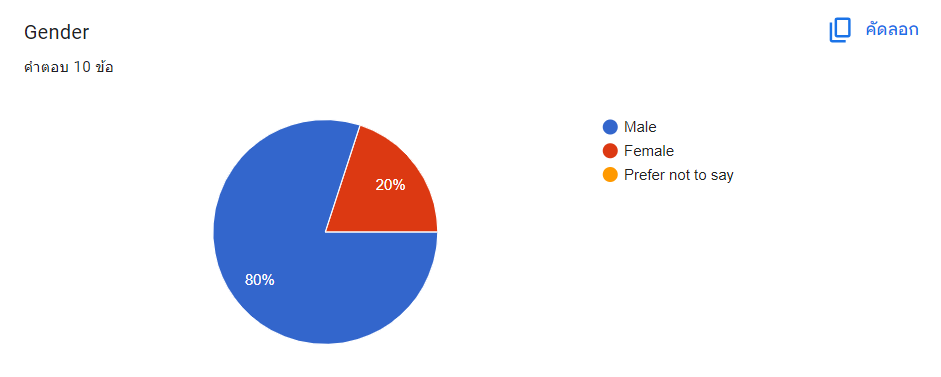
\includegraphics[width=0.8\textwidth]{./img/result/2.png}
    \label{fig:gender}
    \end{center}
\end{subfigure}
\caption{กราฟแสดงอายุและเพศของผู้เข้าร่วมการทดสอบ}
\end{figure}

\begin{figure}[h]
\begin{subfigure}{\textwidth}
    \begin{center}
    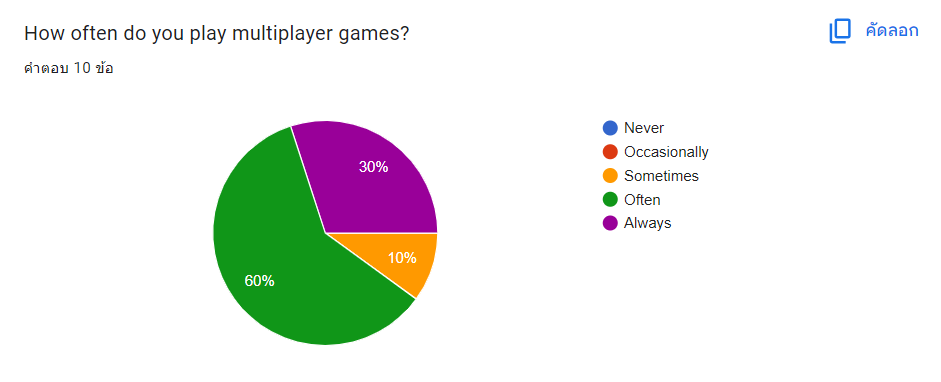
\includegraphics[width=0.8\textwidth]{./img/result/3.png}
    \end{center}
\end{subfigure}
\begin{subfigure}{\textwidth}
    \begin{center}
    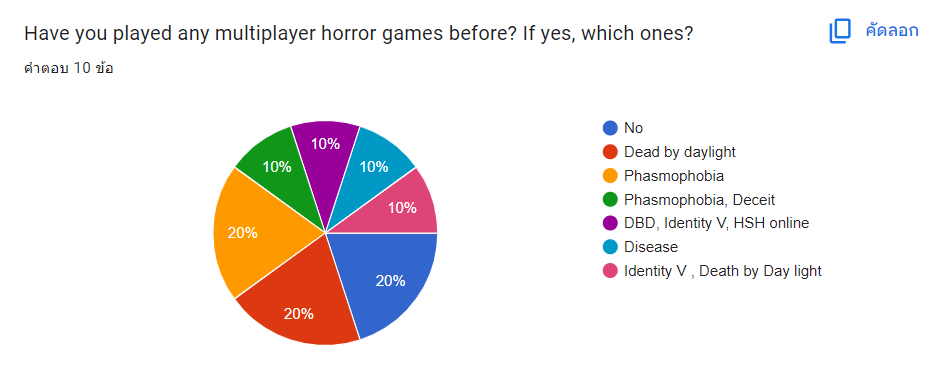
\includegraphics[width=0.8\textwidth]{./img/result/4.png}
    \end{center}
\end{subfigure}
\caption{กราฟแสดงข้อมูลประวัติการเล่นเกมแนว Multiplayer Horror ของผู้เข้าร่วมการทดสอบ}
\end{figure}

\begin{table}[]
    \begin{tabular}{|p{0.65\textwidth}|lllllr|}
    \hline
    \multicolumn{1}{|c|}{\multirow{2}{*}{คำถาม}} &
      \multicolumn{5}{c|}{ระดับการวัดผล} &
      \multicolumn{1}{c|}{\multirow{2}{*}{ค่าเฉลี่ย}} \\ \cline{2-6}
    \multicolumn{1}{|c|}{} &
      \multicolumn{1}{c|}{1} &
      \multicolumn{1}{c|}{2} &
      \multicolumn{1}{c|}{3} &
      \multicolumn{1}{c|}{4} &
      \multicolumn{1}{c|}{5} &
      \multicolumn{1}{c|}{} \\ \hline
    How immersive did you find the game? &
      \multicolumn{1}{c|}{0} &
      \multicolumn{1}{c|}{0} &
      \multicolumn{1}{c|}{5} &
      \multicolumn{1}{c|}{3} &
      \multicolumn{1}{l|}{1} &
      3.56 \\ \hline
    How would you rate your overall enjoyment of the multiplayer horror game? &
      \multicolumn{1}{l|}{0} &
      \multicolumn{1}{l|}{0} &
      \multicolumn{1}{l|}{3} &
      \multicolumn{1}{l|}{7} &
      \multicolumn{1}{l|}{0} &
      3.70 \\ \hline
    How effective were the game's mechanics in creating a sense of tension and fear? &
      \multicolumn{1}{l|}{0} &
      \multicolumn{1}{l|}{2} &
      \multicolumn{1}{l|}{2} &
      \multicolumn{1}{l|}{4} &
      \multicolumn{1}{l|}{2} &
      3.60 \\ \hline
    How well did the game utilize sound effects and music to enhance the horror experience? &
      \multicolumn{1}{l|}{0} &
      \multicolumn{1}{l|}{0} &
      \multicolumn{1}{l|}{1} &
      \multicolumn{1}{l|}{5} &
      \multicolumn{1}{l|}{4} &
      4.30 \\ \hline
    How would you rate the graphical quality and visual atmosphere of the game? &
      \multicolumn{1}{l|}{0} &
      \multicolumn{1}{l|}{0} &
      \multicolumn{1}{l|}{2} &
      \multicolumn{1}{l|}{4} &
      \multicolumn{1}{l|}{4} &
      4.20 \\ \hline
    Considering all aspects of the game, how likely are you to recommend it to a friend? &
      \multicolumn{1}{l|}{0} &
      \multicolumn{1}{l|}{1} &
      \multicolumn{1}{l|}{4} &
      \multicolumn{1}{l|}{4} &
      \multicolumn{1}{l|}{1} &
      3.50 \\ \hline
    How satisfied were you with the pacing of the game? &
      \multicolumn{1}{l|}{0} &
      \multicolumn{1}{l|}{1} &
      \multicolumn{1}{l|}{5} &
      \multicolumn{1}{l|}{3} &
      \multicolumn{1}{l|}{1} &
      3.40 \\ \hline
    \textbf{คะแนนเฉลี่ยความพึงพอใจ} &
      \multicolumn{6}{r|}{3.75} \\ \hline
    \end{tabular}
    \caption{คะแนนจากการทดสอบความพึงพอใจในการเล่น}
\end{table}

\pagebreak

\textbf{ตัวอย่างความคิดเห็นเรื่องความรู้สึกขณะเล่นเกม}
\begin{enumerate}
    \item "บรรยากาศชวนระแวง แต่ก็สนุกและก็ลุ้นดี ตัวละครชวนน่ากลัวเข้ากับเกม"
    \item "Witch - รู้สึกสนุกดีแต่ว่าท่าอ้วกใช้ยากมาก ไม่เคยโดน เดินไปแทบจะจูบ hunter แล้วก็ยังไม่โดน
    Hunter - รู้สึกว่าการทำ objective ไม่ได้ยากเกินไป แต่ว่าตอนสวดทำพิธีนานไปมากๆ ควรลดเวลาลงหน่อย"
    \item "ตื่นเต้นดี งงๆ ตอนแรก แต่ถ้าเล่นไปน่าจะสนุกขึ้น"
    \item "Hunter: ระทึกดีโดยเฉพาะตอนโดน witch ไล่ เกมเพลย์ต้องใช้ความสามารถระดับนึง เช่น การปามีด
    Witch: ค่อนข้างเก่ง โดยเฉพาะท่าชาร์จยิงคลิกขาว ท่าคลิกซ้ายใช้งานยาก"
\end{enumerate}

\textbf{ตัวอย่างความคิดเห็นเรื่องสิ่งที่อยากให้ปรับปรุง}
\begin{enumerate}
    \item "มีให้เห็นว่าเพื่อนเราโดนตีกี่ที ใกล้ตายรึยัง สถานะเป็นยังไง "
    \item "มีแมพเล็กๆ  ให้ดูมุมซ้ายบน"
    \item "ในอนาคตอาจจะมีจำนวนตัวละครในแต่ละเกมส์เพิ่ม"
    \item "สกิลเฉพาะแต่ละตัวละคร"
    \item "ฮันเตอร์กับวิชน่าจะจับคู่แบบห้องที่ไม่เห็นตัวละครต่างฝ่ายกัน "
    \item "มีข้อความกดบอกกันว่าวิชอยู่ใกล้ หรือ ทำอะไรอยู่เป็นต้น"
\end{enumerate}

จากผลการทดสอบ ผู้เล่นมีความพอใจมากที่สุดในเรื่องของเสียงและเพลงประกอบเกมที่ช่วยสร้างเสริมประสบการณ์ที่ระทึกและสยองขวัญ
โดยมีคะแนนเฉลี่ยอยู่ที่ 4.30 จาก 5 ส่วนที่ควรมีการปรับปรุงมากที่สุดคือเรื่องจังหวะของเกม (Pacing) 
ซึ่งมีคะแนนเฉลี่ยอยู่ที่ 3.40 อยู่ในระดับพอใจ ในเรื่องของความสนุกสนานของเกมและการสร้างความตึงเครียดและสยองขวัญให้กับผู้เล่น
มีคะแนนเฉลี่ยอยู่ที่ 3.70 และ 3.60 ตามลำดับ โดยรวมแล้วผู้เล่นมีความพึงพอใจในการเล่นเกม Witch Hunter อยู่ที่ 3.75 จาก 5 อยู่ในระดับพอใจค่อนไปทางพอใจมาก
สรุปได้ว่าเกมนี้จะดีขึ้นอีกถ้ามีการปรับปรุงเรื่องของจังหวะของเกมให้เหมาะสมมากขึ้น ปรับปรุงการใช้งานสกิลให้ตัวละครให้ง่ายขึ้น และแก้ไขข้อบกพร่องต่าง
 ๆ ในระบบเกมที่เกิดขึ้นบางครั้งในระหว่างการทดสอบ
